\documentclass{article}
\usepackage{graphicx} % Required for inserting images
\usepackage{amssymb}
\usepackage{listings}

\title{hetFL}
\author{shamsiiat.abdurakhmanova }
\date{February 2023}

\begin{document}

\maketitle

\section{Numerical experiments}

\subsection{Datasets}

\subsubsection{Synthetic Dataset}

Experiments were performed on a synthetic dataset whose empirical graph $\mathcal {G}$ is partitioned into 3 equal-sized clusters $\mathcal{P} = \{\mathcal{C}^{(1)}, \mathcal{C}^{(2)}, \mathcal{C}^{(3)}\}$, with $|\mathcal{C}^{(1)}|=|\mathcal{C}^{(2)}|=|\mathcal{C}^{(3)}|$. We denote the cluster assignment of node $i \in \mathcal{V}$ by ${c}^{(i)} \in \{1,2,3\}$. The edges in $\mathcal {G}$  are generated via realizations of independent binary random variables ${b}_{i,{i}^{'}} \in \{0,1\}$. These random variables are indexed by pairs $i,{i}^{'}$ of nodes that are connected by an edge $\{i,{i}^{'}\} \in \mathcal{E}$ if and only if ${b}_{i,{i}^{'}}=1$. \\
Two nodes in the same cluster are connected with probability $Prob\{{b}_{i,{i}^{'}}=1\} :={p}_{in}$ if nodes $i,{i}^{'}$ belong to the same cluster. In contrast, $Prob\{{b}_{i,{i}^{'}}=1\} :={p}_{out}$ if nodes $i,{i}^{'}$ belong to different clusters. Every edge in  $\mathcal {G}$ has the same weight, ${A}_{e}=1$ for all $e \in \mathcal{E}$.

Each node $i \in \mathcal {V}$ of the empirical graph $\mathcal {G}$ holds a local dataset $\mathcal {D}_{(i)}$ of the form $\mathcal {D}^{(i)} := \{ ({x}^{(i,1)}, {y}^{(i,1)}), ..., ({x}^{(i,{m}_{i})}, {y}^{(i,{m}_{i})}) \}$. Thus, dataset $\mathcal {D}_{(i)}$ consist of ${m}_{i}$ data points, each characterized by a feature vector $\mathbf{x}^{(i,r)} \in \mathbb{R}^{d}$ and scalar label ${y}^{(i,r)}$, for $r=1,...,{m}_{i}$. The feature vectors $\mathbf{x}^{(i,r)} \sim \mathcal{N}(\mathbf{{\mu}^{(i)}},\mathbf{{\Sigma}^{(i)}})$, are drawn i.i.d. from a multivariate normal distribution with mean vector $\mathbf{\mu}^{(i)}$ and covariance matrix $\mathbf{\Sigma}^{(i)}$. 
Nodes from the same cluster share the same mean vector and covariance matrix, i.e. $\mathbf{\mu}^{(i)} = \mathbf{\mu}^{({i}^{'})}, \mathbf{\Sigma}^{(i)} = \mathbf{\Sigma}^{({i}^{'})}$ if ${c}^{(i)}={c}^{({i}^{'})}$.\\
Mean vector of cluster $\mathcal{C}^{(i)}$, $\mathbf{{\mu}^{(i)}}$, was drawn from a normal standard distribution $N(0,1)$.
Covariance matrix $\mathbf{\Sigma}^{(i)}$ for each cluster was created as follows: samples were drawn from a normal standard distribution $N(0,1)$ to form a square matrix $M$ and covarinace matrix defined as $\mathbf{\Sigma} = M{M}^{T}$ to ensure that matrix is symmetric and positive-semidefinite.\\
The labels of the data points are generated by a noisy linear model
\begin{equation}
{y}^{(i,r)} = (\mathbf{w}^{(i)})^T\mathbf{x}^{(i,r)} + {\varepsilon}^{(i,r)}
\end{equation}

The noise ${\varepsilon}^{(i,r)} \sim \mathcal{N}(0, 1)$, for $i \in \mathcal{V}$ and $r=1,..,{m}_{i}$, are i.i.d. realizations of a normal distribution. The true underlying vector $\mathbf{w}^{(i)} \sim \mathcal{N}(0,1)$ is drawn from a standard normal distribution and is the same for nodes from the same cluster, i.e. $\mathbf{w}^{(i)}=\mathbf{w}^{({i}^{'})}$ if ${c}^{(i)}={c}^{({i}^{'})}$.

Datasets were divided into training and validation subsets by using resampling with replacement. The size of the validation subset was ${m}^{(val)}_{i}=100$. Features of training and validation sets were standardized by removing the mean and scaling to unit variance.

\subsubsection{"Toy" Sklearn Dataset}

In these experiments, empirical graph $\mathcal {G}$ is also partitioned into 3 equal-sized clusters $\mathcal{P} = \{\mathcal{C}^{(1)}, \mathcal{C}^{(2)}, \mathcal{C}^{(3)}\}$, but we used sklearn Python library to create 3 datasets corresponding to 3 clusters. 
First dataset is created with \verb|make_regression()| function with parameters \verb|n_samples=1000| and \verb|n_features=d|. Second and third datasets are  \verb|fetch_california_housing|  and \verb|load_diabetes| with $d$-first features selected for experiments. Training and validation subsets sampling and feature scaling were done in the same way as described in section above.

\subsubsection{Shared Dataset}

Dataset, which predictions are shared across all nodes was formed as follows:
the feature, weight and noise vectors are drawn i.i.d. from a standard normal distribution and labels are generated by a noisy linear model. 

\subsection{Algorithm Implementation}

$\frac{1}{m} \sum_{r=1}^{{m}_{i}}L(({x}^{(i,r)}, {y}^{(i,r)}), {h}^{(i)})  + \frac{\lambda}{{2m}^{'}} \sum_{{i}^{'} \in {\mathcal V}} \sum_{r=1}^{{m}^{'}}{A}_{i,{i}^{'}}L(({x}^{(r)}, {h}^{(i)}({x}^{(r)}), {h}^{({i}^{'})}) $ \\

For $i = {i}^{'}, {A}_{i,{i}^{'}}=0

\subsection{Algorithm Implementation with augmented dataset}

$\frac{1}{(m + n*{m}^{'})} \left[ \sum_{r=1}^{{m}_{i}}L(({x}^{(i,r)}, {y}^{(i,r)}), {h}^{(i)})  + \sum_{{i}^{'} \in {\mathcal V}} \lambda \sum_{r=1}^{{m}^{'}}{A}_{i,{i}^{'}}L(({x}^{(r)}, {h}^{(i)}({x}^{(r)}), {h}^{({i}^{'})})  \right] $ \\

Where $n$ is number of nodes and for $i = {i}^{'}, {A}_{i,{i}^{'}}=0$

\subsection{Experiments}
In these experiments the number of datasets belonging to a cluster is set to 5 and number of features of each local dataset is $d=5$. The sample size of the shared dataset is ${m}^{'}=50$.

All models in this graph are implementation of a linear regression in pytorch with optimizer RMSprop.

\subsubsection{Pytorch linear regression models with varying learning rate.}

Synthetic dataset:

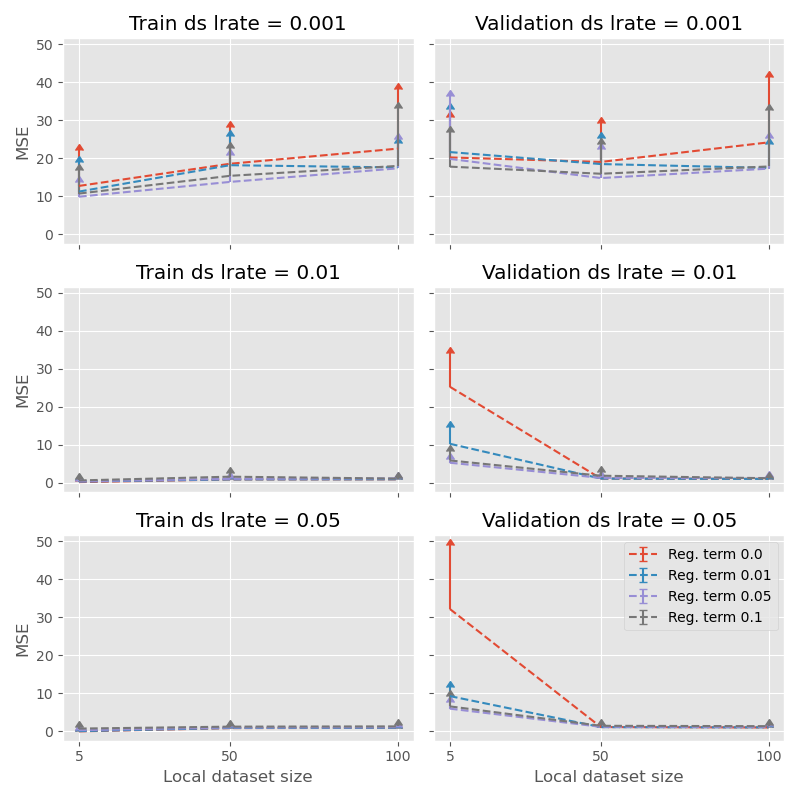
\includegraphics[width=10cm]{linreg_syn_ds_lrate.png}

"Toy" dataset:

\includegraphics[width=10cm]{linreg_toy_ds.png}

\end{document}
